% mnras_guide.tex
%
% MNRAS LaTeX user guide
%
% v3.0 released 22 May 2015
% (version numbers match those of mnras.cls)
%
% Copyright (C) Royal Astronomical Society 2015
% Authors:
% Keith T. Smith (Royal Astronomical Society)

% Change log
%
% v3.0   September 2013 - May 2015
%    First version: complete rewrite of the user guide
%    Basic structure taken from mnras_template.tex by the same author

%%%%%%%%%%%%%%%%%%%%%%%%%%%%%%%%%%%%%%%%%%%%%%%%%%
% Basic setup. Most papers should leave these options alone.
\documentclass[fleqn,usenatbib,useAMS]{mnras}

%%%%% AUTHORS - PLACE YOUR OWN PACKAGES HERE %%%%%

% Only include extra packages if you really need them. Common packages are:
\usepackage{graphicx}	% Including figure files
\usepackage{amsmath}	% Advanced maths commands
\usepackage{amssymb}	% Extra maths symbols
\usepackage{multicol}        % Multi-column entries in tables
\usepackage{bm}		% Bold maths symbols, including upright Greek
\usepackage{pdflscape}	% Landscape pages

%%%%%%%%%%%%%%%%%%%%%%%%%%%%%%%%%%%%%%%%%%%%%%%%%%

%%%%%% AUTHORS - PLACE YOUR OWN MACROS HERE %%%%%%

% Please keep new commands to a minimum, and use \newcommand not \def to avoid
% overwriting existing commands. Example:
%\newcommand{\pcm}{\,cm$^{-2}$}	% per cm-squared
\newcommand{\kms}{\,km\,s$^{-1}$} % kilometres per second
\newcommand{\bibtex}{\textsc{Bib}\!\TeX} % bibtex. Not quite the correct typesetting, but close enough

%%%%%%%%%%%%%%%%%%%%%%%%%%%%%%%%%%%%%%%%%%%%%%%%%%


% Use vector fonts, so it zooms properly in on-screen viewing software
% Don't change these lines unless you know what you are doing
\usepackage[T1]{fontenc}
\usepackage{ae,aecompl}

% MNRAS is set in Times font. If you don't have this installed (most LaTeX
% installations will be fine) or prefer the old Computer Modern fonts, comment
% out the following line
\usepackage{newtxtext,newtxmath}
% Depending on your LaTeX fonts installation, you might get better results with one of these:
%\usepackage{mathptmx}
%\usepackage{txfonts}

%%%%%%%%%%%%%%%%%%% TITLE PAGE %%%%%%%%%%%%%%%%%%%

% Title of the paper, and the short title which is used in the headers.
% Keep the title short and informative.
\title[MNRAS]{The Fates of Merging Supermassive Black Holes and A Proposal for a New Class of X-Ray Sources}

% The list of authors, and the short list which is used in the headers.
% If you need two or more lines of authors, add an extra line using \newauthor
\author[]{
Charles Zivancev$^{1}$\thanks{Contact e-mail: \href{mailto:csz2104@columbia.edu}{csz2104@columbia.edu}},
Jeremiah Ostriker$^{1}$,
Andreas H.W. K\"upper$^{2}$
\\
% List of institutions
$^{1}$Department of Astronomy, Columbia University, 550 West 120th Street, New York, NY 10027, USA\\
$^{2}$Hubble Fellow\\
}
% These dates will be filled out by the publisher
\date{Last updated 2019 Nov 09; in original form 2019 November 9}

% Enter the current year, for the copyright statements etc.
\pubyear{2019}


% Don't change these lines
\begin{document}
\label{firstpage}
\pagerange{\pageref{firstpage}--\pageref{lastpage}}
\maketitle



\begin{abstract}
We perform N-body simulations on 11 galaxies extracted from a cosmological simulation of hierarchical structure formation with total mass in the range $10^{12} M_{\sun} < M < 10^{13} M_{\sun}$ from 4 $\gid$ z $\gid$ 0.  After mergers, we track the dynamical evolution of the orbiting black holes (BHs) around their host central BHs.  Of the 86 orbiting BHs, we find that 36 merge with their host central BHs, 13 are ejected from their respective host galaxies, and 37 are still orbiting at the end of the simulations.  Across all galaxies, 33 BHs are kicked to a higher orbit after close interactions with the central BHs, after which only one of them merged with their hosts.  These orbiting BHs should be detectable by their anomalous (not LMXRB) spectra.  The x-ray luminosities of the orbiting massive BHs at z=0 are in the range $10^{25}-10^{43}$ $erg\ s^{-1}$, with an undetectable median value $10^{32}$ $erg\ s^{-1}$.  However, the most luminous $\sim$$5\%$ should be detectable.
\end{abstract}


\begin{keywords}
Galaxy: kinematics and dynamics
\end{keywords}




\section{Introduction}\label{sec:introduction}
What happens to the massive black holes centrally located in galaxies when those galaxies merge with others?  There are three possibilities: they merge, they are ejected, or they remain in orbit in the merged galaxy.  Combinations of these options are also possible with the spin induced kick at merger leading to an ejection or extended orbit of the merged black hole.  We now know from pulsar timing measurements (\citet{2008MNRAS.390..192S}, \citet{2018ApJ...856...42S}, \citet{2016APS..APRR18003T}) that the gravitational wave background is probably too low for most galaxy mergers (mass-weighted) (but see \cite{2018NatCo...9..573M}) to lead to BH mergers, but the outcome remains uncertain.  We will argue in this paper that a very common outcome--especially for the lower mass black holes--is for the injected objects to remain as orbiting X-ray sources in normal massive galaxies waiting to be identified by current observational techniques.

There is no "final parsec problem," and the opposite problem of too many BH mergers is also avoided when it is realized that we are dealing with a small N-body system rather than a series of two-body problems (cf \citet{2018MNRAS.473.3410R}).

How common are mergers of massive black holes?  For the galaxies themselves we know that minor mergers are frequent from the observed (\citet{2010ApJ...718L..73V}, \citet{2008ApJ...677L...5V}, \citet{2019MNRAS.484..595M}) evolution of the size and mass of these systems, but assuming that all galaxy mergers lead to SMBH mergers overpredicts the observations of gravitational waves from the pulsar timing arrays (PTAs) (\citet{2008MNRAS.390..192S}, \citet{2009MNRAS.394.2255S}, \citet{2013MNRAS.433L...1S}, \citet{2014ApJ...789..156M}, \citet{2015ApJ...799..178K}, \citet{2018ApJ...856...42S}, \citet{2018arXiv180403143I}).  However, we do not often see multiple SMBHs at the centers of massive ellipticals (but see \citet{2016MNRAS.463.2145C}).  So, what does happen?  One paper (\citet{2018MNRAS.473.3410R}) has indicated that dynamical interactions among multiple orbiting black holes, which will eject a non-negligible fraction of the mass, may solve this problem.  The present paper also addresses this purported dynamical solution, focusing attention on the large fraction of lower mass black holes that remain to be detected as they orbit in massive galaxies.  What we argue in this paper is that, as a result of the N-body interactions among the infalling black holes, some are ejected, some remain in extended orbits and some (the few most massive ones) do in fact merge, but these do not exceed the PTA limits, and some of the orbiting ones might be detectable via their ability to accrete gas and emit radiation.

Here we look at the merger history of 11 exemplary galaxies across the galaxy mass spectrum extracted from a cosmological simulation of hierarchical structure formation. We investigate how, after merging with incoming galaxies, SMBHs sink into the cores of the hosts and interact with the resident black hole. We show that gravitational interactions of multiple SMBHs are most probable in high-mass galaxies with total mass $10^{12} M_{\sun} < M < 10^{13} M_{\sun}$. Galaxies with lower masses have too few mergers with SMBH hosting galaxies. Galaxies with higher masses are more extended, making dynamical friction processes less efficient and hence failing to drive SMBHs into the host galaxy core.

This paper is organized as follows: in Section \ref{sec:methods} we describe the cosmological simulations from which we use the merger history to set up our idealized numerical simulations. We present the few-body integration code, \textsc{AR-Chain} that we used for our simulations of SMBH dynamics, and the modifications we made to this code in order to deal with a host galaxy's gravitational potential. In Section \ref{sec:results}, we show the results of our 11 exemplary simulations of galaxies growing with time and acquiring new SMBHs. We analyze how the SMBHs spiral into the core of their new host galaxies due to dynamical friction, and how interactions with the host black hole and other orbiting BHs leads to near-ejections or mergers. We then estimate the X-ray luminosities expected of the orbiting black holes.  The final Section \ref{sec:conclusions} contains a discussion of the results and our conclusions.

\section{Methods}\label{sec:methods}
%\begin{figure}
%\begin{center}
%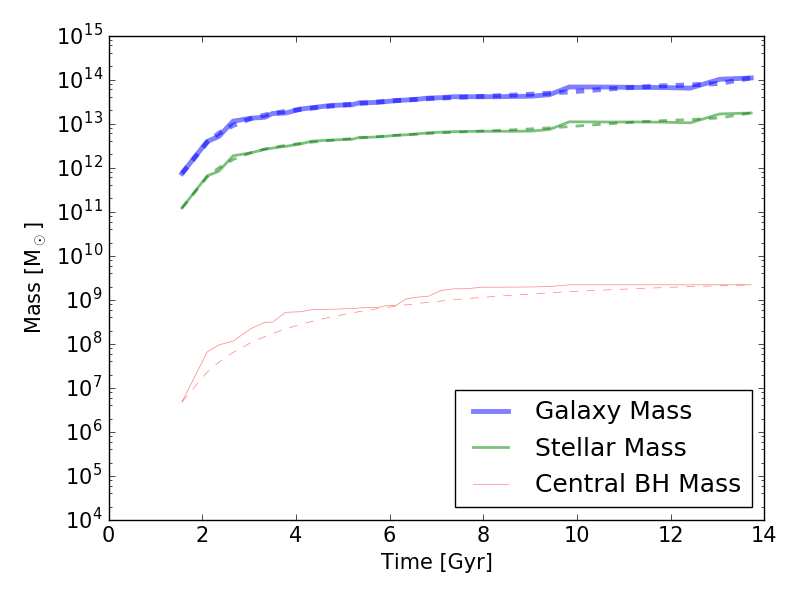
\includegraphics[width=0.45\textwidth]{plots/Masses_plot_galaxy_1.png}
%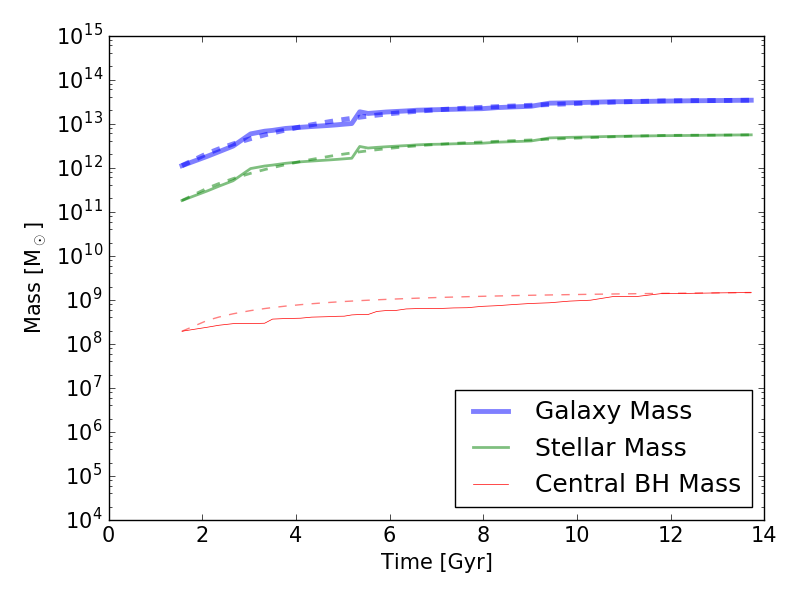
\includegraphics[width=0.45\textwidth]{plots/Masses_plot_galaxy_65.png}\\
%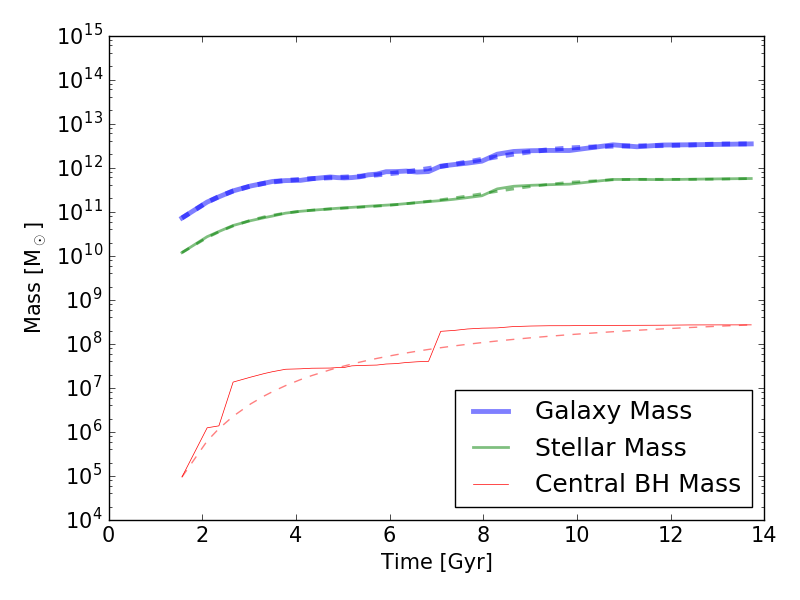
\includegraphics[width=0.45\textwidth]{plots/Masses_plot_galaxy_187.png}
%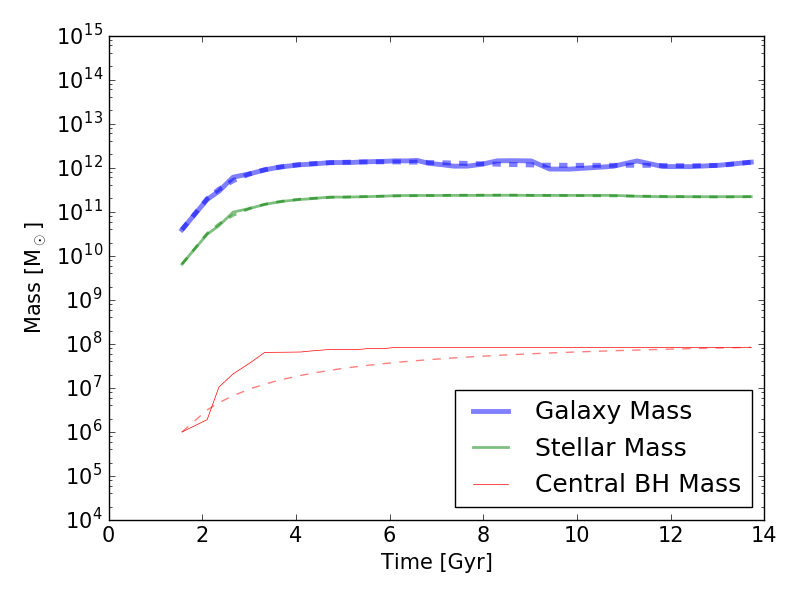
\includegraphics[width=0.45\textwidth]{plots/Masses_plot_galaxy_217.png}\\
%\caption{default}
%\label{default1}
%\end{center}
%\end{figure*}

\subsection{Overview of simulation}
Our simulations focus on elliptical galaxies with central SMBHs. The galaxies were given a dark matter background potential using the Stone-Ostriker profile (\citet{2015ApJ...806L..28S}), which is a three-parameter potential-density pair, whose quantities such as density, potential, and binding energy can be written in closed form, having a profile similar to that of a truncated isothermal sphere.  The galaxies were evolved from $4 > z > 0$.  Orbiting black holes were periodically introduced into the "host" galaxy following mergers and their dynamical interaction with the background potential and central SMBH were followed, as described further below.

For the numerical simulations presented here, we used a modified version of the algorithmic chain integrator \textsc{AR-Chain} developed by \citet{2006MNRAS.372..219M}. It uses algorithmic chain regularization for high-precision integration of few-body dynamics, and is capable of handling velocity-dependent forces efficiently. It includes relativistic post-Newtonian terms up to order PN2.5 \citep{2008AJ....135.2398M}.


\subsection{Merger tree Data}
The merger tree data that was used as the input to our simulations is the result of previous work by \citet{2011ApJ...741...99C, 2011ApJ...742L..33C, 2012ApJ...753...17C, 2012ApJ...748..121C, 2013ApJ...770..139C} (hereafter Cen(+11)), \citet{2012MNRAS.425..641L} (hereafter Lackner(+12)), and \citet{2015ApJ...799..178K} (hereafter Kulier(+15)).  A brief synopsis of the work that led to our input data is described below.

Cen(+11) studied the "cosmic downsizing" effect (e.g., \citet{1996AJ....112..839C}) using high-resolution large-scale hydrodynamic galaxy formation simulations.  His work produced physical parameters for galaxies such as position, velocity, total mass, stellar mass, gas mass, mean formation time, mean stellar metallicity, mean gas metallicity, SFR, luminosities, etc.

Lackner(+12), using Cen(+11)'s work as a basis, created galactic merger trees that compared the properties of in situ and accreted stellar mass of galaxies at redshift snapshots between $4 > z > 0$.

Kulier(+15) furthered the merger tree data produced by Lackner(+12) by estimating the evolution of the SMBH population, based on assumptions about the relationship between the properties of SMBHs and those of their host galaxies.

The primary data we extracted from the above work was organized as follows:
\begin{itemize}
    \item Galactic properties - Each galaxy was distinguished by an id number, with properties such as stellar mass, dark matter mass, central black hole id number, and orbiting black hole id numbers, recorded at 37 redshift slices between $4 > z > 0$.
    \item Black Hole properties - Each black hole was also distinguished by an id number, with properties such as seed mass, accreted mass, its host galaxy id number, and time after $z=4$ at which the black hole entered its host galaxy, if it was not the central black hole.
\end{itemize}

The merger tree data from Lackner(+12) and Kulier\-(+15) provided 1,830 galaxies in total.  However, not all the galaxies were suitable for our simulations.  We placed further requirements as follows:
\begin{itemize}
\item The galaxies had to exist through the entire simulation ($4 > z > 0$).  If they merged with other galaxies, they had to have been the "surviving" galaxy at each merger.
\item They had to have accumulated orbiting black holes by $z = 0$.
\end{itemize}

The above criteria narrowed the field of eligible galaxies down to 51.  In considering time and resources, we chose the top 13 galaxies in terms of number of black holes to run the simulations.  The black holes in these galaxies accounted for nearly $84{\%}$ of all orbiting black holes across all the galaxies, so it represented a reasonable balance between completeness and efficiency.

The following cosmological parameters were used in our simulations, consistent with both Lackner(+12) and Kulier(+15):   $\Omega_M = 0.28$, $\Omega_b = 0.046$, $\Omega_\Lambda = 0.72$, $\sigma_8 = 0.82$, $H_0 = 100h^{-1}Mpc^{-1} = 70 km s^{-1} Mpc^{-1}$, and $n = 0.96$.

\subsubsection{Stellar Mass Adjustment}
As we will explain further in Section \ref{Galaxy background potential}, in our simulations orbiting black holes are inserted into the host galaxy at the effective radius, $R_e$, which is partially dependent on stellar mass, $M_*$ (see equation \ref{re}).  For every doubling of the stellar mass, $M_*$, $R_e$ increases by a factor of 1.66.  Additionally, the velocity dispersion at the effective radius, $\sigma(R_e)$, which is used to set the parameter $r_h$ of our dark matter profile, is also dependent on $M_*$.  In this case, a doubling of $M_*$ would increase $\sigma(R_e)$ by a factor of 1.15.  These variations have direct effects on the ability of the orbiting black holes to merge with the central black hole, and thus can affect our merger statistics and resulting characteristic strain calculations, and therefore it is important to estimate our stellar masses with reasonable accuracy.

In cosmological simulations it is common to overproduce stellar mass, with a general over-efficiency in the range of 2-4 times those measured in observations (\citet{1996ApJS..105...19K}, \citet{2010MNRAS.404.1111G}, \citet{2010ApJ...725.2312O}).  One typical reason cited for this overproduction is a lack or underestimation of supernova feedback effects in the form of thermal and/or kinetic energy.  However, even when thermal energy from supernova feedback is considered, the effects may be reduced due to the energy being quickly radiated away by rapidly cooling surrounding gas (\citet{1996ApJS..105...19K}).  A second common reason for overproduction of stars in cosmological simulations is a lack of modeling for AGN feedback, which may be responsible for solving the phenomenon called the "cooling flow paradox" (\citet{2001MNRAS.321L..20F}) that suppresses star formation. 

Lackner(+12), which is the source of our stellar masses, noted that the efficiency of star formation in their simulations, defined as $f_*=M_*/M_{DM}(\Omega_{DM}/\Omega_b)$, was approximately 0.6.  Compared with the expected range of $0.10 \loa f_* \loa 0.15$ that they referenced from \citet{2012ApJ...746...95L}, their stellar masses were a factor of roughly 4 times greater.

We also compared the stellar masses from Lackner\-(+12) to  observational and abundance matching data from \citet{2018AstL...44....8K}. Figure \ref{fig:stellar1} is a partial, approximate, replication of their Figure 11 (abundance matching line).  We rescaled our stellar masses at $z=0$ in a lognormal manner about the line in order to match the observed data.  Table \ref{table:gal_char} shows the original and rescaled stellar masses.

\begin{figure}
%\begin{center}
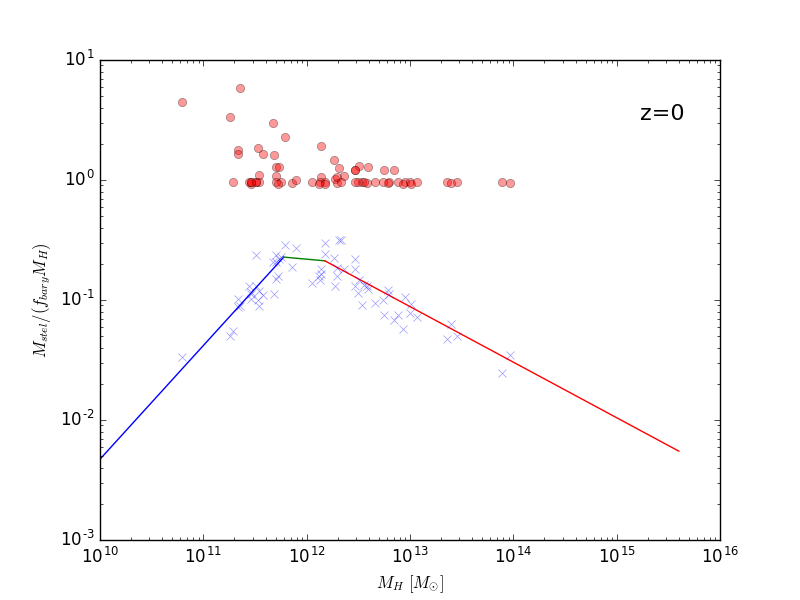
\includegraphics[width=0.5\textwidth]{plots/stellar_to_halo_ratio.png}
\caption{Approximation of Figure 11 from \citet{2018AstL...44....8K}.  Purple dots shown are examples of our rescaled stellar masses}
\label{fig:stellar1}
%\end{center}
\end{figure}

\begin{table}
\begin{center}
\caption{Galaxy characteristics at z=0. Units are M$\sun$.}
\begin{tabular} {|c | c | c| c|}
\hline
$M_{DM}$ & $M_{CBH}$ & $M_{*} (orig.)$ & $M_{*} (rescaled)$ \\
\hline
 2.85 $\times 10^{13}$ 	&	 1.46 $\times 10^9$	&	5.58 $\times 10^{12}$ 	&	3.30 $\times 10^{11}$  \\
 2.48 $\times 10^{13}$ 	&	 2.40 $\times 10^9$	&	4.80 $\times 10^{12}$ 	&	2.25 $\times 10^{11}$  \\
 2.29 $\times 10^{13}$ 	&	 1.22 $\times 10^9$	&	4.46 $\times 10^{12}$ 	&	2.68 $\times 10^{11}$  \\
 1.18 $\times 10^{13}$ 	&	 3.62 $\times 10^9$	&	2.32 $\times 10^{12}$ 	&	2.83 $\times 10^{11}$  \\
 1.03 $\times 10^{13}$ 	&	 9.85 $\times 10^9$	&	1.96 $\times 10^{12}$ 	&	1.62 $\times 10^{11}$  \\
 1.00 $\times 10^{13}$ 	&	 9.32 $\times 10^9$	&	1.95 $\times 10^{12}$ 	&	2.49 $\times 10^{11}$  \\
 8.92 $\times 10^{12}$ 	&	 5.60 $\times 10^9$	&	1.74 $\times 10^{12}$ 	&	3.20 $\times 10^{11}$  \\
 8.56 $\times 10^{12}$ 	&	 6.86 $\times 10^9$	&	1.62 $\times 10^{12}$ 	&	1.83 $\times 10^{11}$  \\
 6.94 $\times 10^{12}$ 	&	 2.02 $\times 10^9$	&	1.72 $\times 10^{12}$ 	&	1.51 $\times 10^{11}$  \\
 6.29 $\times 10^{12}$ 	&	 1.22 $\times 10^9$	&	1.23 $\times 10^{12}$ 	&	1.87 $\times 10^{11}$  \\
 1.84 $\times 10^{12}$ 	&	 2.21 $\times 10^9$	&	5.52 $\times 10^{11}$ 	&	6.42 $\times 10^{10}$  \\
\hline
\end{tabular}
\end{center}
\label{table:gal_char}
\end{table}

\subsection{Simulation Physics}
In this section, we describe the underlying physics of our simulations, including choice of galaxy background potential, BH diffusion through the galaxy, and gravitational wave kicks as a result of mergers.

\subsubsection{Galaxy background potential} \label{Galaxy background potential}
In order to model the dark matter halo distribution in our simulations, we used the Stone-Ostriker profile (\citet{2015ApJ...806L..28S}), which is a three-parameter potential-density pair.  Quantities such as density, potential, and binding energy can be written in closed form.  It is essentially an analytic form of a finite, cored isothermal mass distribution:
\begin{equation} \label{jerry}
\rho(r) = \frac{\rho_c}{(1+r^2/r_{c}^2)(1+r^2/r_{h}^2)}.
\end{equation}
Here $\rho_c$ is the central density, $r_c$ is the core radius, and $r_h$ is the outer halo radius.

In order to parameterize this profile, $r_c$ was given an initial value of 100 pc, which is reasonable for a cored massive system.  To calculate $r_h$, we began by using the stellar mass to calculate the velocity dispersion at the galaxy's effective radius.  In Kulier(+15), the galaxy's effective radius $R_{e}$ and velocity dispersion $\sigma(R_e)$ at the effective radius are:
\begin{equation} \label{re}
R_{e} = 2.5 kpc\left(\frac{M_*}{10^{11}M_{\odot}}\right)^{0.73}(1+z)^{-0.98},
\end{equation}
\begin{equation} \label{sig}
\sigma(R_{e}) = 190km/s\left(\frac{M_{*}}{10^{11}M_{\odot}}\right)^{0.2}(1+z)^{0.47},
\end{equation}

We can then equate the value for $\sigma({R_e})$ obtained from Equation \ref{sig} to the analytic expressions for $\sigma(R_{e})$ in the Stone-Ostriker profile (Eqns 9 and A1-A4).  The only unknown is $r_h$, which we can solve for using a simple recursive Newton method.  Whether $\sigma_{near}$ or $\sigma_{far}$ is used from Stone-Ostriker is determined by whether $R_e$ is less than or greater than $\sqrt{r_c r_h}$.

The central density, $\rho_c$, can be found from Equation 5 in Stone-Ostriker:
\begin{equation} \label{rhoc}
M_{tot} = \frac{2\pi^2r_{c}^2r_{h}^2\rho_c}{r_h+r_c},
\end{equation}
where $M_{tot}$ is the total dark matter mass.

At each iteration in the code, $r_h$ is updated according to the stellar mass and Equations \ref{re} and \ref{sig}.  The core radius, $r_c$, is recalculated only if an orbiting black hole enters within $r_c$.  The work done by diffusion, as described in Section \ref{psd} is calculated, the total potential energy and dynamical friction are updated, and $r_c$ is solved for from Equation 8 in Stone-Ostriker based on conservation of energy.

\subsubsection{Phase-space diffusion} \label{psd}
Weak encounters with background stars will let the SMBHs diffuse through phase space while they are orbiting within the gravitational potential of the galaxy. The diffusion can be expressed as change in velocity of an SMBH by $\Delta \vec{v}$ per unit time. We can split this change into a component along the direction of motion of the SMBH, and one perpendicular to that. Following \citet{2008gady.book.....B}, the diffusion coefficients can be expressed as 
\begin{eqnarray}\label{eq:df}
D[\Delta v_\parallel] & = & -\frac{4\pi G^2\rho(r)M_\bullet\ln\Lambda}{\sigma^2}f(\chi),\\
D[(\Delta v_\parallel)^2] & = & \frac{4\sqrt{2}\pi G^2\rho(r)M_\bullet\ln\Lambda}{\sigma}\frac{f(\chi)}{\chi},\\
D[(\Delta \vec{v}_\bot)^2] & = & \frac{4\sqrt{2}\pi G^2\rho(r)M_\bullet\ln\Lambda}{\sigma}\left[\frac{\mbox{erf}(\chi)-f(\chi)}{\chi}\right],
\end{eqnarray} 
where $\Delta v_\parallel \equiv \Delta \vec{v}\cdot\vec{v}/v$ is the velocity change in direction of motion, and $\Delta \vec{v}_\bot \equiv \Delta \vec{v} - \Delta v_\parallel \cdot\vec{v}/v$ is the velocity change perpendicular to the direction of motion. Here, $M_\bullet$ is the mass of the black hole, and $\chi = \frac{v}{\sqrt{2}\sigma(r)}$. The function $f(\chi)$ is given by 
\begin{equation}
f(\chi) \equiv \frac{1}{2\chi^2}\left(\mbox{erf}(\chi)-\frac{2\chi}{\sqrt{\pi}}\exp\left(-\chi^2\right)\right).
\end{equation}
We approximate the factor $\Lambda$ in the Coulomb logarithm as
\begin{equation}
\Lambda \equiv \left(\frac{M_{NSC}}{M_\bullet}\right)\left(\frac{r}{r_h}\right).
\end{equation}
We can identify Equation \ref{eq:df} as the dynamical friction term. The second term introduces a variance of the friction term, and even allows the SBHs to be accelerated when the velocity of a SBH is sufficiently small. The third term introduces a change in velocity perpendicular to the direction of motion of the SBH. It is a randomly oriented vector, and hence causes the SBHs to depart from smooth orbits due to the small random velocity kicks. The last two terms will establish that the SBHs are ultimately in energy equipartition with the background stars.
The velocity changes $\Delta v_\parallel$ and $\Delta\vec{v}_\bot$ per unit time $\Delta t$ can be computed with the above equations. Both changes are normally distributed, where the mean, $\mu$, and the variance, $\Sigma$, of the distributions are given by
\begin{eqnarray}
\mu_\parallel &=& D[\Delta v_\parallel]\Delta t,\\
\Sigma_\parallel &=& D[(\Delta v_\parallel)^2]\Delta t,\\
\mu_\bot &=& 0,\\
\Sigma_\bot &=& D[(\Delta \vec{v}_\bot)^2]\Delta t.
\end{eqnarray}
We compute the diffusion coefficients for each black hole at each time step, and modify its velocity on a Monte Carlo basis. For each time step we draw a random orientation before adding the perpendicular velocity change to the respective SBH. Hence, the SBH's modified velocity, $v_f$, is computed using
\begin{eqnarray}
\vec{v}_f &=& \vec{v}_0 + \Delta v_\parallel \hat{v}_\parallel + \Delta v_\bot \hat{v}_\bot,\\
\Delta v_\parallel &=& \mathcal{N}(\mu_\parallel, \Sigma_\parallel),\\
\Delta v_\bot &=& \mathcal{N}(\mu_\bot, \Sigma_\bot).
\end{eqnarray}
The change of energy, $\mbox{d}E_{BH}$, of the orbiting black hole due to phase-space diffusion is given back to the stellar background potential, with $\mbox{d}E = -\mbox{d}E_{BH}$. As a consequence of this energy transfer, inspiralling black holes will cause an expansion of the stellar system. For this purpose we calculate the change in potential energy, $\mbox{d}W$, of the stellar system using
\begin{eqnarray}
E &=& T + W = \frac{1}{2}W,\\
\mbox{d}W &=& -2\,\mbox{d}E_{BH},
\end{eqnarray}
where we made use of the virial theorem $2T+W =0$. With this change in potential energy we can calculate a new radius for the stellar background potential at each integration step. For the Plummer sphere the new scale radius can be calculated as
\begin{equation}
a_{new} = a\left(1+\frac{32a\,\mbox{d}W}{3\pi GM_{NSC}^2}\right)^{-1}.
\end{equation}

\subsubsection{Gravitational wave recoils}
The code \textsc{AR-Chain} includes post-Newtonian terms up to order 2.5. The SMBHs can therefore merge via gravitational wave emission. We include gravitational wave recoils following the prescription outlined in Kulier(+15), which is based on the fitting formula by \citet{2012PhRvD..85h4015L}.  We assume that a merger will be inevitable when the separation between two SMBHs becomes smaller than 1.0x the Schwarzschild radius. At the moment of the merger, we also assume that the spin vectors of the two SBHs are randomly aligned.

A result of the anisotropic emission of gravitational waves is that the merged binary often experiences a linear kick in the opposite direction of the emission of the GW due to conservation of linear momentum. This kick can result in velocities of the merged binary from approximately $200-5000\ km s^{-1}$ (see \citet{2007PhRvL..98w1101G}, \citet{2007PhRvL..98i1101G}, \citet{2007PhRvL..98w1102C}, \citet{2011PhRvL.107w1102L}).  In our simulations, the binaries never stray more than a few tens of parsecs from the nucleus of the host galaxies.

Black holes can also eject each other via strong three-body interactions. We remove SBHs from the simulations once they move beyond $r_h$, assuming that it will take them more than a Hubble time to find their way back into the center of the host galaxy, or that they have achieved escape velocity.

\subsection{Simulation setup}
For each galaxy in the simulations, we only used black holes that would theoretically have merged with the center of the host galaxy within a dynamical friction time, $t_{fric}$, of less than 100 times a Hubble time, with $t_{fric}$ defined from \citet{2008gady.book.....B} as:
\begin{equation}\label{tfric}
    t_{fric} = \frac{19}{6}\left(\frac{R_e}{5kpc}\right)^2\frac{\sigma_{eff}}{200km\,s^{-1}}\frac{10^8\,M_{\odot}}{M_{bh}} \text{  Gyr}.
\end{equation}
The orbiting black holes were injected into their host galaxy at redshift z, at a distance from the galactic center of $R_{e}$ (Equation \ref{re}) following galaxy mergers.  Their initial velocity was arbitrarily chosen to be circular, $v_c = \sqrt{GM(R_e)/R_e}$, with $v_x$, $v_y$, and $v_z$ randomly chosen.

\section{Results}\label{sec:results}
Here we review the primary results of our simulations, focusing on the various interactions of the orbiting black holes with their host SMBHs and the final luminosity characteristics of those that did not merge.

\subsection{Mergers, Ejections/Kicks and Orbiting SMBHs}

\subsubsection{Overview of Results}\label{sec:results_overview}
Figure \ref{fig:meosmbh} shows the distribution of merged, ejected and orbiting black holes across all galaxy simulations as a function of guest black hole mass.

Of the 86 SMBHs used for the simulations, 36 black holes merged with their respective host black hole within a Hubble time, 37 remained orbiting at the end of the simulations, and 13 were ejected from their galaxies as a result of sufficiently large kicks due to three-body interactions with the host and other black holes.

Given the log distribution of masses, one can see the general trend of larger mass BHs ($\goa\, 10^7\, M_{\odot}$) tending to merge with their respective host BH, while lower mass BHs continue to wander at $z=0$.  However, there is some overlap with some BHs greater than $10^7\, M_{\odot}$ still orbiting and those less than $10^7\, M_{\odot}$ having merged.

\subsubsection{Mergers}\label{sec:mergers}
The tendency of larger mass black holes to merge with their host can perhaps be more clearly seen by looking at the merger mass ratio between the incoming black hole and the host.  Figure \ref{fig:q_merge_fraction} displays the fraction of galaxy mergers that result in black hole mergers versus the merger mass ratio, defined as $m_2/m_1$, where $m_2$ is the orbiting black hole and $m_1$ is the host black hole.  The plot monotonically increases with increasing mass ratio, reaching nearly unity for mass ratio of $10^{-1}$, meaning nearly all galaxy mergers with a black hole mass ratio greater than $10^{-1}$ resulted in the orbiting black hole merging with the host.

In figure \ref{fig:time_to_merge} we present the time it took for the merging guest black holes to merge with their host.  As can be seen in the plot, although there is a fair amount of variation, the general trend is a decreasing time to merge as orbiting black hole mass increases.

\subsubsection{Kicked, Ejected and Orbiting Black Holes}\label{sec:kicked_orbiting}
Of the 37 orbiting black holes at $z=0$, 18 of them were kicked to higher orbits at some point in their traversal of their host galaxy.  If one counts the 13 ejected black holes, then of the 50 SMBHs that had not eventually merged with their host, 32 of them were kicked out of the galactic core as a result of three-body interactions.  If they did not merge, it was not for a lack of effort.

Figure \ref{fig:kicked_stats} shows the mass distribution of kicked and not-kicked black holes, including those that merged and those that did not merge.  The vast majority of larger SMBHs ($\goa\, 10^7\, M_{\odot}$) were not kicked to higher orbits nor ejected from their galaxies, which at least partly explains why most of the merged SMBHs are in the greater mass range.  In contrast, most of the SMBHs below $10^7\, M_{\odot}$ are kicked (with a few of them being ejected).  In our simulations, no black holes that are kicked to higher orbits ever returned to merge with their central host SMBH.

Figure \ref{fig:mvr} is a realization of the final radii of the remaining wandering black holes at $z=0$.  There does not appear to be a correlation between mass and final radius.  However, it is evident from the plot that all but one of the black holes that had not been kicked by $z=0$ have mostly approached and entered within the galactic core radius, $r_c$.

\begin{figure}
\begin{center}
\includegraphics[width=0.5\textwidth]{plots/"Summary Results All Galaxies".png}
\caption{Histogram of merged, ejected, and orbiting SMBHs at z=0 as a function of BH mass.  Colored arrows along x-axis represent median masses of respective sets.}
\label{fig:meosmbh}
\end{center}
\end{figure}

\begin{figure}
\begin{center}
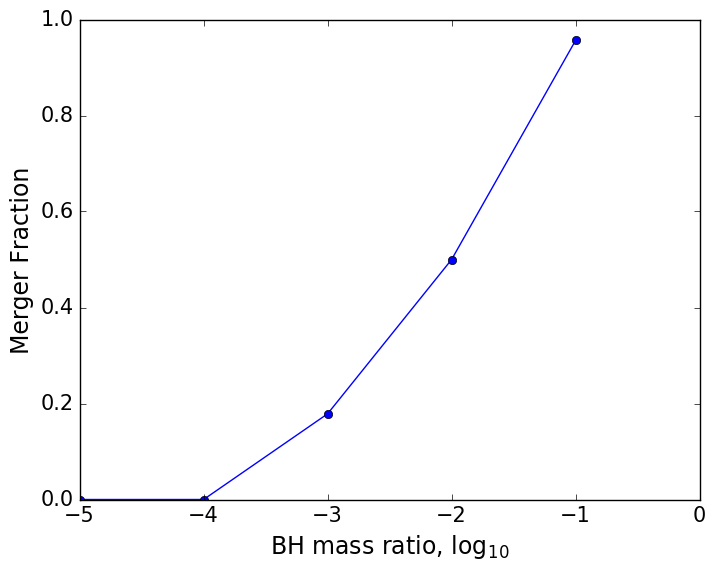
\includegraphics[width=0.5\textwidth]{plots/q_merger_fraction.png}
\caption{Fraction of BHs that merge with the central BH as a function of the BH mass ratio.  Each point represents the fraction of galaxy mergers that led to BH mergers for each BH merger ratio bin.  Note that a "bin" at each point is comprised of the mass ratio at that point up to, but not including, the next point on the x-axis.}
\label{fig:q_merge_fraction}
\end{center}
\end{figure}

\begin{figure}
\begin{center}
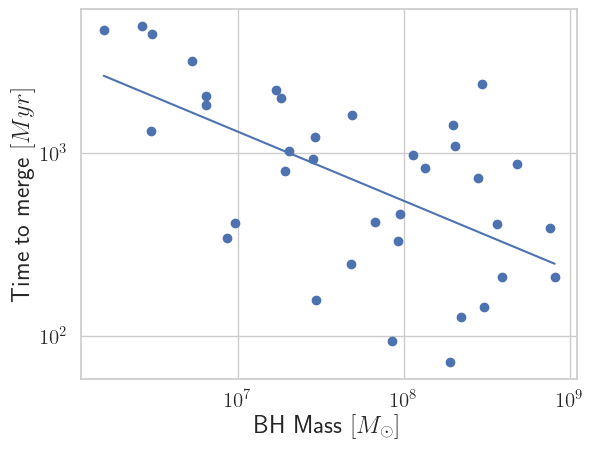
\includegraphics[width=0.5\textwidth]{plots/time_to_merge.png}
\caption{Time required for BHs to merge with host SMBH after galaxy merger.  Form for fitted line is $-0.379M_{BH}+5.766$ in log-log space.}
\label{fig:time_to_merge}
\end{center}
\end{figure}

\begin{figure}
\begin{center}
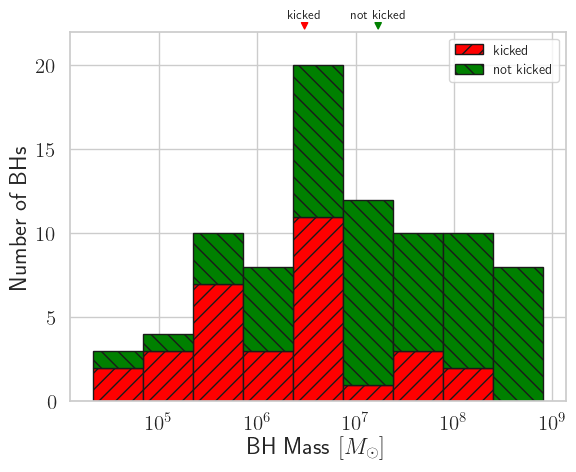
\includegraphics[width=0.5\textwidth]{plots/kicked_stats.png}
\caption{Histogram of kicked and not-kicked SMBHs at z=0.  Colored arrows along x-axis represent median masses of respective sets.}
\label{fig:kicked_stats}
\end{center}
\end{figure}

\begin{figure}
\begin{center}
\includegraphics[width=0.5\textwidth]{plots/"Final Radius v Mass of Orbiting BHs".png}
\caption{Final Radii of remaining orbital black holes at z=0.}
\label{fig:mvr}
\end{center}
\end{figure}

\begin{figure}
\vspace{20pt}%
\begin{center}
\includegraphics[width=0.5\textwidth]{plots/"Lx of our Galaxies compared to Babyk data".png}
\caption{X-ray luminosity of hot gas in our galaxies, compared to those from \citet{2018ApJ...857...32B}.}
\label{fig:galgas1}
\end{center}
\end{figure}

\subsection{Galaxy Gas X-Ray Luminosity}
We compute the x-ray luminosity of the hot gas in the galaxies, adapting Equation 26 from \citet{2012ApJ...754..125C}. In lieu of summing over discrete particles, we use the beta model of the gas as defined in our equation \ref{beta_model} and integrate:
\begin{equation}
\begin{aligned}
    L_x ={} \frac{1.2 \times 10^{-24}}{(\mu m_p)^2}\left(\frac{kT_x}{1keV}\right)^{1/2}\rho_0^{2}\;4{\pi} \\
    \int_{0}^{\infty}\frac{r^2}{(1+r^2/r_c^2)^{3}}\;dr\text{  erg s}^{-1}.
\end{aligned}
\end{equation}

The integral evaluates to ${\pi}r_c^3/16$.  $m_p$ is the mass of a proton and $\mu$ is the mean molecular weight.  To calculate $\mu$, we use metallicity $Z=2Z_{\odot}=0.0268$, mass fraction of Helium $Y=Y_{\odot}=0.2485$, and mass fraction of Hydrogen $X=0.7247$.  This results in $\mu=0.606$.

\subsection{Black Hole Luminosity}
The x-ray temperature versus sigma relation from Table 2 of  \citet{2018ApJ...857...32B} was fitted according to:
\begin{equation}
    T_x = 10^{2.50*log(\sigma) - 6.06} \text{  kev}.
\end{equation}
Central gas density, ${\rho}_0$ was also fitted from Table 3 of \citet{2018ApJ...857...32B} according to:
\begin{equation}
    \rho_0 = 10^{0.6*log(\sigma) - 25} \text{  g cm}^{-3}.
\end{equation}
The core radius of the gas model, ${r_c}$ is:
\begin{equation}
    r_c = 10^{2.1*log(\sigma) - 5.3} \text{  kpc}.
\end{equation}
Local gas density ${\rho}$ is obtained from the isothermal beta model (\citet{1962AJ.....67..471K}, \citet{1976A&A....49..137C}, \citet{1978A&A....70..677C}):
\begin{equation} \label{beta_model}
    \rho = \frac{\rho_0}{(1+r^2/r_c^2)^{1.5}} \text{  g cm}^{-3}.
\end{equation}

Gas sound speed, $c_s$, was obtained from:
\begin{equation}
    C_s = \sqrt{1.67T_x/m_p} \text{  km s}^{-1},
\end{equation}
where $m_p$ is the proton mass.

The net black hole mass accretion rate is approximated by \citet{2018MNRAS.476.1412I} and \citet{2019arXiv190202349I}:
\begin{equation}
    \dot{M}_{acc} = \frac{4{\pi}G^2M^2\rho}{(C_s^2+v^2)^{3/2}} \text{  M}_\odot \text{ Myr}^{-1},
\end{equation}
where M is black hole mass, G is the gravitational constant, and v is the black hole velocity.

Finally, the black hole x-ray luminosity is estimated from:
\begin{equation}
    L_x = 0.01\dot{M}_{acc}c^2 \text{  erg s}^{-1}.
\end{equation}

The Eddington limit is defined as:
\begin{equation}
    L_{edd} = 1.26 \times 10^{38} (M/M_{\odot}) \text{  erg s}^{-1}.
\end{equation}

%\begin{figure}
%\begin{center}
%\includegraphics[width=0.45\%textwidth]{plots/"Final %Luminosities of Orbiting %BHs".png}
%\caption{Luminosities of %Orbiting BHs at z=0}
%\label{fig:loobhs}
%\end{center}
%\end{figure}

\begin{figure}
\begin{center}
\includegraphics[width=0.5\textwidth]{plots/"luminosities_final".png}
\caption{Luminosity of orbiting BHs at z=0 as per Inayoshi (2019).}
\label{fig:loobhs}
\end{center}
\end{figure}

\begin{figure}
\begin{center}
\includegraphics[width=0.5\textwidth]{plots/"Final Luminosities using Kohei factor".png}
\caption{Xray Luminosity Distribution of Orbiting BHs at z=0.}
\label{fig:ldobhs}
\end{center}
\end{figure}


\subsection{Central Black Hole Influence}
Within the influence radius of the central black hole, which is defined as the radius at which the total mass of the galaxy within that radius (stars + dark matter) equals the mass of the central black hole, the gas density is much higher than otherwise, and equation \eqref{beta_model} cannot be used in the region where the BH Kepler potential dominates.  Starting with the equation for hydrostatic equilibrium, assuming isothermality,
\begin{equation}
    C_{s}^2\frac{dln\rho}{dr}= -\frac{GM(r)}{r^2},
\end{equation}
we can integrate with respect to r, leading to 
\begin{equation}
    ln\frac{\rho}{\rho_1} = \frac{GM}{C_{s}^2}\left(\frac{1}{r} - \frac{1}{r_1}\right),
\end{equation}
where $\rho$ is the gas density at the location of the wandering black hole, $\rho_1$ is the density at the radius where the central black hole mass equals the galaxy mass, $r$ is the distance of the wandering black hole from the center, and $r_1$ is the radius where the central black hole mass equals the galaxy mass.

Figure \ref{fig:wui} shows the difference in luminosity when taking into account the influence of the central black hole for the wandering black holes that were within the influence radius.  In all cases, the final luminosity is higher than the original luminosity.
\begin{figure}
\begin{center}
\includegraphics[width=0.5\textwidth]{plots/"Comparison of L_x versus radius with and without BH Influence".png}
\caption{Difference in x-ray luminosity of wandering black holes within the influence radius of the central black hole.  Red dots are the originally calculated luminosity, not taking the CBH influence into account.  Green dots are the final luminosities, taking the central BH influence into account.}
\label{fig:wui}
\end{center}
\end{figure}

\section{Conclusions}\label{sec:conclusions}
We performed N-body simulations on 11 galaxies ranging in mass between $10^{12}$ M$_{\sun}$ < M < $10^{13}$ M$_{\sun}$, from 4 $\gid$ z $\gid$ 0.  A total of 86 orbiting black holes were followed in our simulations, resulting in 42$\%$ mergers with their host galaxy, while another 43$\%$ remained in orbit at $z=0$.  Those remaining orbiting black holes had x-ray luminosities in the range of $10^{25}-10^{43}$ $erg\ s^{-1}$.  The median luminosity of $10^{32} erg\ s^{-1}$ would be undetectable with present instruments, although the top $5\%$ most luminous from this set could be detectable.

\section{Acknowledgements}
The authors would like to thank Andrea Kulier and Claire Lackner for providing merger tree data. AHWK acknowledges support by NASA through Hubble Fellowship grant HST-HF-51323.01-A awarded by the Space Telescope Science Institute, which is operated by the Association of Universities for Research in Astronomy, Inc., for NASA, under contract NAS 5-26555.

%%%%%%%%%%%%%%%%%%%%%%%%%%%%%%%%%%%%%%%%%%%%%%%%%%

%%%%%%%%%%%%%%%%%%%% REFERENCES %%%%%%%%%%%%%%%%%%

% The best way to enter references is to use BibTeX:

\bibliographystyle{mnras}
\bibliography{biblio}


% Don't change these lines
\bsp	% typesetting comment
\label{lastpage}
\end{document}

% End of mnras_guide.tex